\documentclass[11pt,letterpaper]{article}

\usepackage[spanish]{babel}
\usepackage[utf8]{inputenc}
\usepackage[T1]{fontenc}

\usepackage{amsmath,amssymb,amsthm,mathtools}
\usepackage{geometry}
\usepackage{enumitem}
\usepackage{tikz}
\usepackage{pgfplots}
\usepackage{xcolor}
\usepackage{hyperref}
\usepackage{graphicx}
\usepackage{float}
\usepackage{booktabs}
\usepackage{tcolorbox}
\tcbuselibrary{theorems,skins}
\pgfplotsset{compat=1.18}
\usetikzlibrary{arrows.meta,calc,positioning,babel}

\geometry{margin=2.4cm}
\setlength{\parindent}{0pt}
\setlength{\parskip}{6pt}
\hypersetup{colorlinks=true, linkcolor=blue, urlcolor=blue}

% ── Colores ────────────────────────────────────────────────────────────────
\definecolor{azul}{RGB}{37,99,235}
\definecolor{rojo}{RGB}{220,38,38}
\definecolor{verde}{RGB}{22,163,74}
\definecolor{gris}{RGB}{71,85,105}
\definecolor{fondodef}{RGB}{239,246,255}
\definecolor{fondoteo}{RGB}{240,253,244}
\definecolor{fondoobs}{RGB}{255,251,235}

% ── Entornos ───────────────────────────────────────────────────────────────
\newtcbtheorem[number within=section]{definicion}{Definición}{
  colback=fondodef, colframe=azul, fonttitle=\bfseries,
  separator sign none, description delimiters parenthesis,
  label type=definition}{def}

\newtcbtheorem[number within=section]{teorema}{Teorema}{
  colback=fondoteo, colframe=verde, fonttitle=\bfseries,
  separator sign none, description delimiters parenthesis,
  label type=theorem}{teo}

\newtcbtheorem[number within=section]{observacion}{Observación}{
  colback=fondoobs, colframe=orange!80!black, fonttitle=\bfseries,
  separator sign none}{obs}

\newtheorem{ejemplo}{Ejemplo}[section]

\newcommand{\dd}{\,d}
\newcommand{\cte}{\operatorname{cte}}



\begin{document}
\begin{center}
  {\LARGE\bfseries Tarea 3}\\[6pt]
  {\large UEA: Modelación Matemática I}\\[4pt]
  {\large Autor: Alejandro Cruz López}
\end{center}

\bigskip
\noindent\rule{\textwidth}{0.5pt}
\bigskip

% ============================================================
\section{Marco teórico: serie de Taylor vectorial}
% ============================================================

Nos ocupamos de funciones de la forma
\[
  F:\mathbb{R}^2\longrightarrow\mathbb{R}^2,
  \qquad
  F(x,y)=\bigl(f(x,y),\,g(x,y)\bigr),
\]
donde $f$ y $g$ son suficientemente diferenciables en una vecindad del punto
$P=(x_0,y_0)$.
La idea fundamental es que toda función suave puede aproximarse localmente
por su parte lineal, y esta aproximación —la \emph{serie de Taylor truncada}—
es la herramienta central del análisis de sistemas dinámicos no lineales
(véase Strogatz \cite{strogatz2018}, \S6.3).

\begin{definicion}{Serie de Taylor de $F$ alrededor de $P$}{}
Sea $F=(f,g):\mathbb{R}^2\to\mathbb{R}^2$ de clase $C^\infty$ en una vecindad
de $P=(x_0,y_0)$. Introduciendo el desplazamiento
$\mathbf{u}=(x-x_0,\,y-y_0)^{\!\top}$, la \textbf{serie de Taylor vectorial}
de $F$ alrededor de $P$ es
\[
  F(x,y)
  = F(x_0,y_0)
  + J_F(x_0,y_0)\,\mathbf{u}
  + \tfrac{1}{2}\,\mathcal{H}[F](x_0,y_0)\,\mathbf{u}^{\otimes 2}
  + \cdots,
\]
donde $J_F$ es la \emph{matriz jacobiana} y $\mathcal{H}[F]$ denota el término
de segundo orden formado con las hessianas de $f$ y $g$.
\end{definicion}

Definimos cada objeto:

\textbf{Jacobiana:}
\[
  J_F(x_0,y_0)
  = \begin{pmatrix}
      \dfrac{\partial f}{\partial x} & \dfrac{\partial f}{\partial y}\\[8pt]
      \dfrac{\partial g}{\partial x} & \dfrac{\partial g}{\partial y}
    \end{pmatrix}_{\!(x_0,\,y_0)}.
\]

\textbf{Término de segundo orden:} para cada componente $\varphi\in\{f,g\}$,
\[
  \tfrac{1}{2}\,\mathbf{u}^{\top} H_\varphi(x_0,y_0)\,\mathbf{u},
  \qquad
  H_\varphi = \begin{pmatrix}
    \varphi_{xx} & \varphi_{xy}\\
    \varphi_{yx} & \varphi_{yy}
  \end{pmatrix}_{\!(x_0,\,y_0)}.
\]

Por tanto, la expansión hasta orden dos queda
\begin{align}
  f(x,y) &= f_0
    + f_x\,(x-x_0) + f_y\,(y-y_0)\notag\\
    &\quad + \tfrac{1}{2}\bigl[f_{xx}(x-x_0)^2
      + 2f_{xy}(x-x_0)(y-y_0)
      + f_{yy}(y-y_0)^2\bigr] + \cdots,\label{eq:taylor_f}\\[4pt]
  g(x,y) &= g_0
    + g_x\,(x-x_0) + g_y\,(y-y_0)\notag\\
    &\quad + \tfrac{1}{2}\bigl[g_{xx}(x-x_0)^2
      + 2g_{xy}(x-x_0)(y-y_0)
      + g_{yy}(y-y_0)^2\bigr] + \cdots,\label{eq:taylor_g}
\end{align}
donde todos los coeficientes se evalúan en $(x_0,y_0)$.

\begin{teorema}{Linealización local (Strogatz \S6.3)}{}
Sea $\mathbf{x}^*$ un punto fijo del sistema $\dot{\mathbf{x}}=F(\mathbf{x})$,
es decir, $F(\mathbf{x}^*)=\mathbf{0}$. Entonces el término constante de la
serie de Taylor se anula y la dinámica local está dominada por la parte lineal:
\[
  \dot{\mathbf{u}} = J_F(\mathbf{x}^*)\,\mathbf{u} + O(\|\mathbf{u}\|^2),
\]
donde $\mathbf{u}=\mathbf{x}-\mathbf{x}^*$. Para \textbf{equilibrios hiperbólicos}
(ningún eigenvalor de $J_F(\mathbf{x}^*)$ tiene parte real nula), los eigenvalores
determinan completamente la naturaleza cualitativa del equilibrio.
Si algún eigenvalor es puramente imaginario, la linealización no basta y
se requiere un análisis no lineal adicional.
\end{teorema}


% ============================================================
\section{Ejemplo 1: sistema de Lotka--Volterra}
% ============================================================

\begin{ejemplo}
Consideremos el sistema depredador-presa
\[
  \begin{cases}
    \dot{P} = rP - aPD,\\[4pt]
    \dot{D} = -\gamma D + \delta a PD,
  \end{cases}
\]
con parámetros $r=1$, $a=0.5$, $\gamma=0.75$, $\delta=0.5$.
En clases hemos visto que este sistema posee el equilibrio interior
\[
  P^* = \frac{\gamma}{\delta a} = 3,
  \qquad
  D^* = \frac{r}{a} = 2.
\]
Definimos $F=(f,g)$ con $f(P,D)=rP-aPD$ y $g(P,D)=-\gamma D+\delta aPD$.

\textbf{Jacobiana en $(P^*,D^*)$:}
\[
  J_F(P^*,D^*)
  = \begin{pmatrix}
      r - aD^* & -aP^*\\
      \delta a D^* & -\gamma + \delta a P^*
    \end{pmatrix}
  = \begin{pmatrix} 0 & -\tfrac{3}{2}\\[4pt] \tfrac{1}{2} & 0 \end{pmatrix}.
\]

Como $F(P^*,D^*)=\mathbf{0}$, la serie de Taylor alrededor de $(P^*,D^*)$
hasta orden uno es
\[
  F(P,D)
  = \begin{pmatrix} 0 & -\tfrac{3}{2}\\[4pt] \tfrac{1}{2} & 0 \end{pmatrix}
    \begin{pmatrix} P - 3\\ D - 2 \end{pmatrix}
  + O\!\left(\|(P-3,\,D-2)\|^2\right).
\]

\textbf{Eigenvalores:} el polinomio característico de $J_F$ es
$\lambda^2 + \tfrac{3}{4} = 0$, de donde $\lambda = \pm i\dfrac{\sqrt{3}}{2}$.
Son puramente imaginarios, lo que indica un \emph{centro} en la linealización.
Sin embargo, como los eigenvalores no son hiperbólicos (parte real nula),
la linealización por sí sola no garantiza que el equilibrio sea un centro
en el sistema no lineal; se requiere un análisis adicional.
En efecto, Lotka--Volterra admite una cantidad conservada que confirma
la existencia de órbitas cerradas alrededor de $(P^*,D^*)$ (Strogatz, \S6.3).

\textbf{Término de segundo orden.} Calculamos las segundas derivadas:
$f_{PP}=0$, $f_{PD}=-a$, $f_{DD}=0$, $g_{PP}=0$, $g_{PD}=\delta a$,
$g_{DD}=0$. Por tanto, las hessianas de $f$ y $g$ son
\[
  H_f = \begin{pmatrix} 0 & -a\\ -a & 0 \end{pmatrix},
  \qquad
  H_g = \begin{pmatrix} 0 & \delta a\\ \delta a & 0 \end{pmatrix}.
\]
Así, la expansión completa hasta orden dos es
\begin{align*}
  f(P,D) &= -\tfrac{3}{2}(D-2) - \tfrac{1}{2}(P-3)(D-2),\\
  g(P,D) &= \tfrac{1}{2}(P-3) + \tfrac{1}{4}(P-3)(D-2).
\end{align*}
Dado que $f$ y $g$ son polinomios cuadráticos, esta expansión es \emph{exacta}:
no existen términos de orden superior.

\end{ejemplo}

\begin{figure}[H]
  \centering
  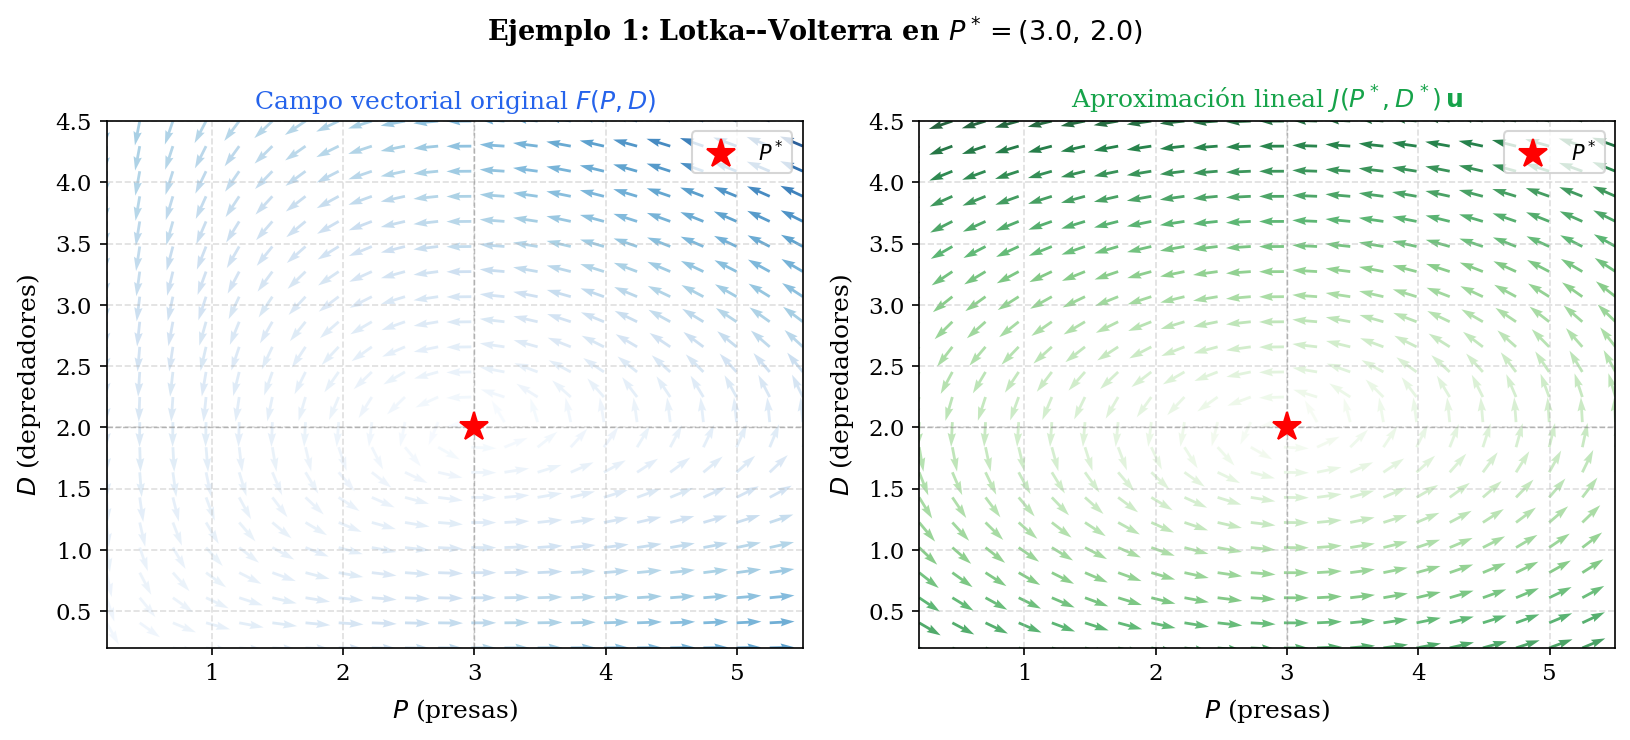
\includegraphics[width=\textwidth]{fig_lotka_volterra.png}
  \caption{Campos vectoriales del sistema de Lotka--Volterra original (izquierda)
  y de su aproximación lineal $J_F(P^*,D^*)\,\mathbf{u}$ (derecha).
  La estrella roja marca el equilibrio $(P^*,D^*)=(3,2)$.
  Nótese que el campo linearizado reproduce fielmente la estructura local
  (rotación pura), pero diverge del original lejos del equilibrio.}
  \label{fig:lv}
\end{figure}

% ============================================================
\section{Ejemplo 2: competencia logística (Volterra)}
% ============================================================

\begin{ejemplo}
En clases hemos visto modelos de dos poblaciones en competencia.
Consideremos el sistema (Strogatz, \S6.4):
\[
  \begin{cases}
    \dot{x} = x(3 - x - 2y),\\[4pt]
    \dot{y} = y(2 - x - y).
  \end{cases}
\]
Definimos $F=(f,g)$ con $f(x,y)=x(3-x-2y)$ y $g(x,y)=y(2-x-y)$.

\textbf{Equilibrio interior:} resolviendo $F(x^*,y^*)=\mathbf{0}$ con
$x^*,y^*>0$, obtenemos $x^*=1$, $y^*=1$.

\textbf{Jacobiana en $(1,1)$:}
las derivadas parciales son
\[
  f_x = 3-2x-2y,\quad f_y = -2x,\quad
  g_x = -y,\quad g_y = 2-x-2y.
\]
Evaluando en $(1,1)$:
\[
  J_F(1,1) = \begin{pmatrix} -1 & -2\\ -1 & -1 \end{pmatrix}.
\]

La serie de Taylor alrededor de $(1,1)$ hasta orden uno es
\[
  F(x,y)
  = \begin{pmatrix} -1 & -2\\ -1 & -1 \end{pmatrix}
    \begin{pmatrix} x-1\\ y-1 \end{pmatrix}
  + O\!\left(\|(x-1,\,y-1)\|^2\right).
\]

\textbf{Eigenvalores:}
$\lambda^2+2\lambda-1=0$, de donde
$\lambda = -1 \pm \sqrt{2}$.
Tenemos $\lambda_1 = -1+\sqrt{2}>0$ y $\lambda_2=-1-\sqrt{2}<0$:
eigenvalores reales de signo opuesto, luego $(1,1)$ es un
\emph{punto silla} inestable (Strogatz, \S6.3).

\textbf{Segundas derivadas:}
$f_{xx}=-2$, $f_{xy}=-2$, $f_{yy}=0$;
$g_{xx}=0$, $g_{xy}=-1$, $g_{yy}=-2$.

Las hessianas son
\[
  H_f = \begin{pmatrix} -2 & -2\\ -2 & 0 \end{pmatrix},
  \qquad
  H_g = \begin{pmatrix} 0 & -1\\ -1 & -2 \end{pmatrix}.
\]
La expansión hasta orden dos queda
\begin{align*}
  f(x,y) &= -(x-1) - 2(y-1) - (x-1)^2 - 2(x-1)(y-1),\\
  g(x,y) &= -(x-1) - (y-1) - (x-1)(y-1) - (y-1)^2.
\end{align*}
Al igual que en el Ejemplo~1, ambos sistemas son cuadráticos, por lo que
la expansión es exacta.

\end{ejemplo}

\begin{figure}[H]
  \centering
  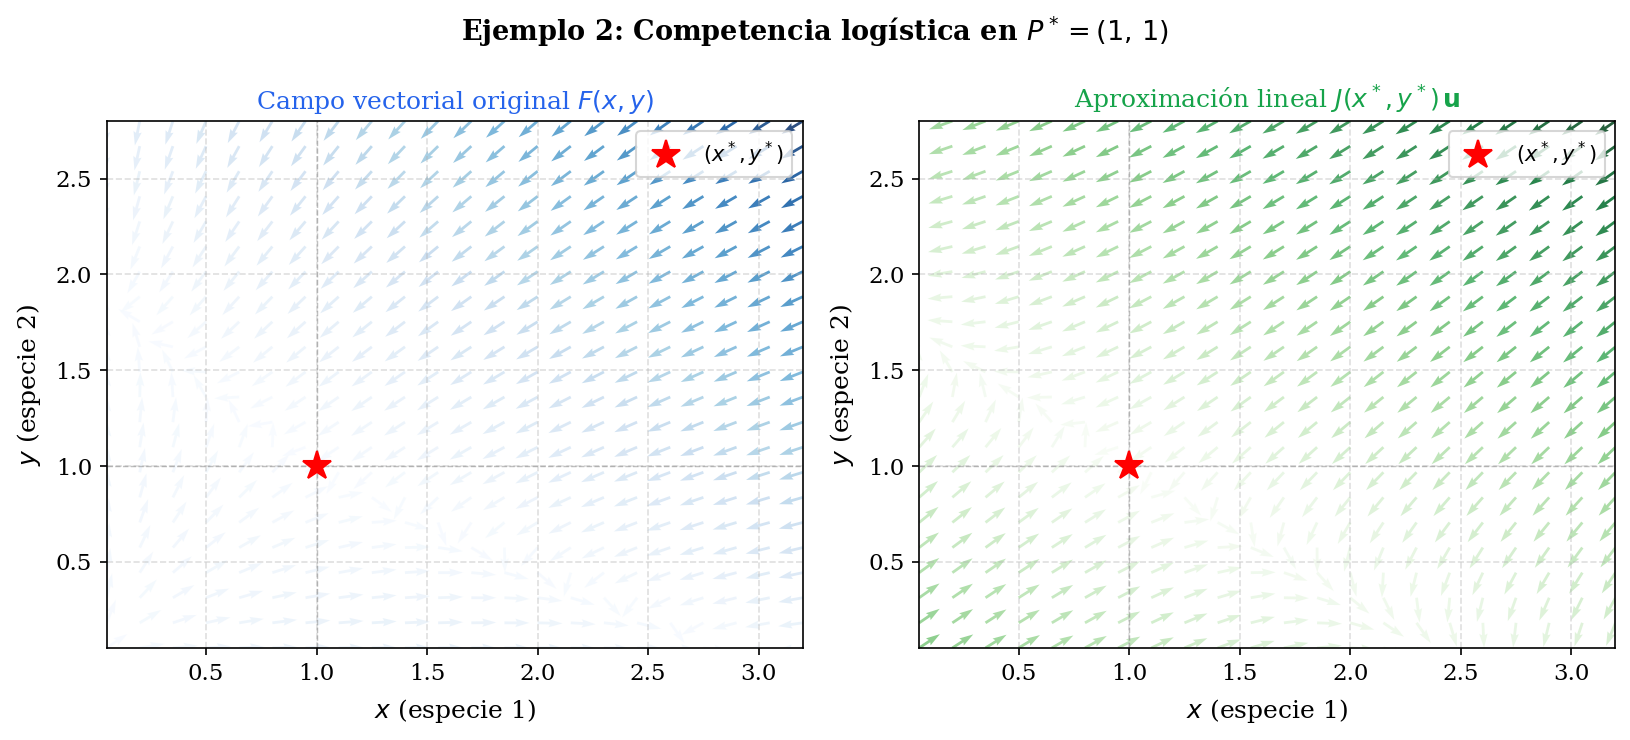
\includegraphics[width=\textwidth]{fig_logistico.png}
  \caption{Campos vectoriales del sistema de competencia logística original
  (izquierda) y de su aproximación lineal $J_F(x^*,y^*)\,\mathbf{u}$ (derecha).
  La estrella roja marca el equilibrio $(x^*,y^*)=(1,1)$.
  La estructura de punto silla es claramente visible en ambos campos cerca
  del equilibrio; la linealización la captura con precisión local.}
  \label{fig:log}
\end{figure}


% ──────────────────────────────────────────────────────────────
\begin{thebibliography}{9}
\bibitem{strogatz2018}
  S.~H.\ Strogatz,
  \emph{Nonlinear Dynamics and Chaos: With Applications to Physics, Biology,
  Chemistry, and Engineering}, 2nd~ed.
  CRC Press, 2018.
  Secciones \S6.3 y \S6.4.
\end{thebibliography}

\end{document}
